\usepackage{subfigure}


% ͼ
%\begin{figure}
%\begin{minipage}[t]{0.5\linewidth}
%\centering
%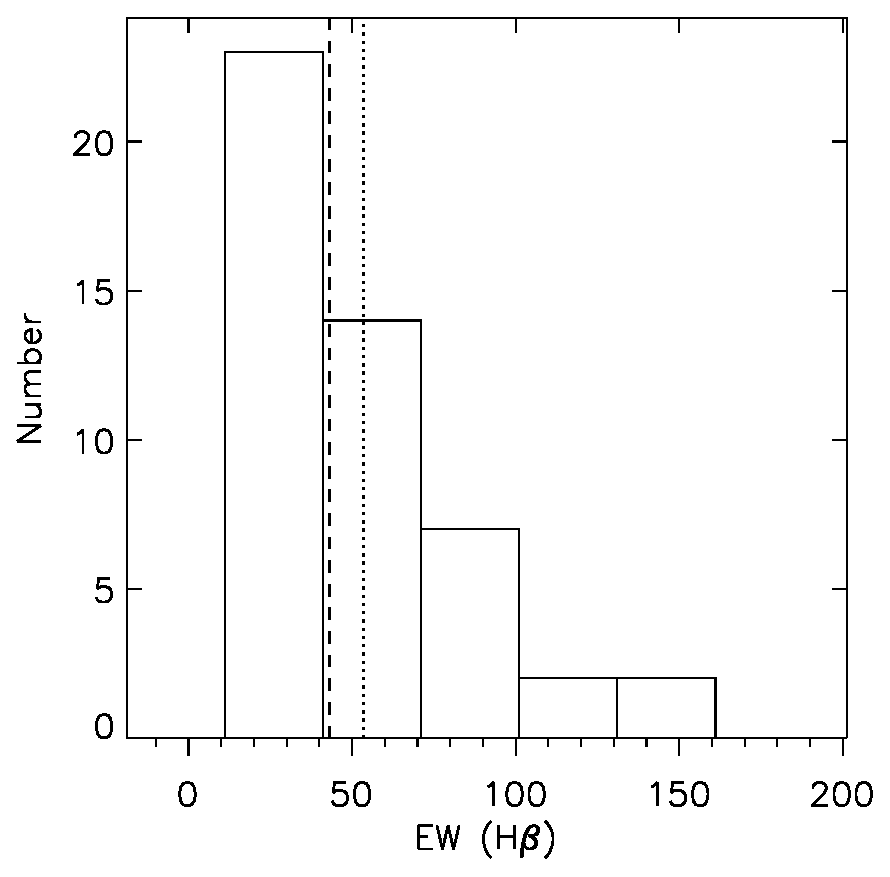
\includegraphics[width=2.2in]{fig1.eps}
%\caption{fig1}
%\label{fig:side:a}
%\end{minipage}%
%\begin{minipage}[t]{0.5\linewidth}
%\centering
%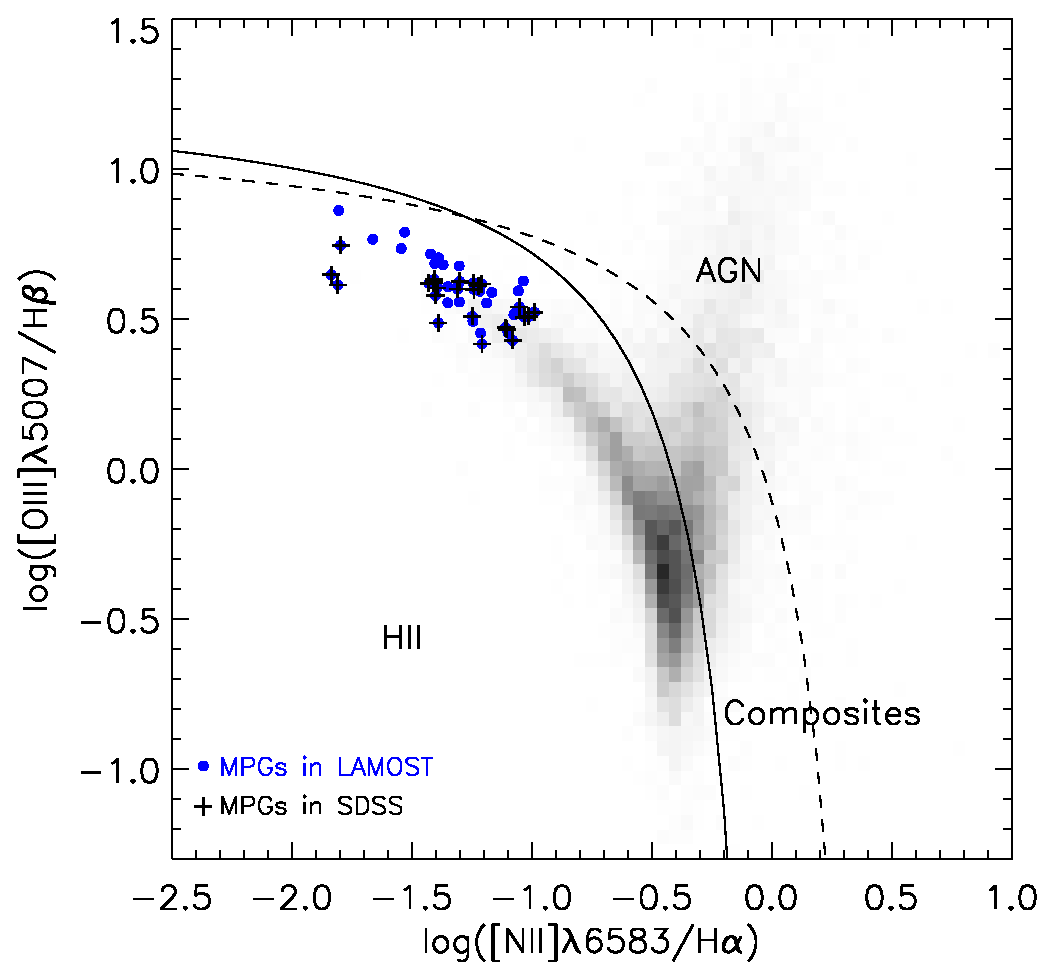
\includegraphics[width=2.2in]{fig2.eps}
%\caption{fig2}
%\label{fig:side:b}
%\end{minipage}
%\end{figure}
\usepackage{graphicx}
\usepackage{url}
\usepackage{pslatex}
\usepackage{bm}
%\usepackage[comma,numbers,square,sort&compress]{natbib} [1,2,3,..]
%\usepackage{cite}[1]-[4]
\usepackage{amsmath,amssymb,amsthm}  %~\\ڶ֤ȻµĻ
\usepackage{paralist}%[flushleft] ʹб
%\usepackage{ntheorem}  ԶõһЩµĶ

%%%%%% ʹ㷨ģ
\usepackage{algorithm}
\usepackage{algorithmic}        %õĺҪԼ
\usepackage{multirow}
\renewcommand{\algorithmicrequire}{\textbf{Initialization:}}   %ijɺС
\renewcommand{\algorithmicensure}{\textbf{Iteration:}}
\renewcommand{\algorithmiclastcon}{\textbf{Output:}} %Used for the algorithm list


%\begin{algorithm}[htb]         %㷨Ŀʼ
%\caption{The proposed algorithm}             %㷨ı
%\label{alg_THong}                  %㷨һǩж㷨
%\begin{algorithmic}[1]
%\REQUIRE ~\\
%Sparsify dictionary matrix $\bm\Psi$, initialize $\bm\Phi_0$ to a random matrix, and the number of iterations: $Iter_{outer}$ and $Iter_{inner}$.
%\lastcon ~\\          %OUTPUT
%  Projection matrix $\bm\Phi$.
%\ENSURE
%\STATE {$\bm\Phi\leftarrow\bm\Phi_0$}
%\FOR {$l=1$ {\bf to} $Iter_{outer}$}
%\STATE ${\bm G_t}\leftarrow \bm\Psi^\mathcal T\bm\Phi^\mathcal T\bm\Phi\bm\Psi$\label{ap1}
%\STATE Update $\bm G_t$:
%\STATE $\text{diag}({\bm G_t})\leftarrow \bm 1$
%\FORALL { $i\neq j$}
%\STATE
%\en
%{\bm G_t(i,j)}\leftarrow
%\left\{\begin{array}{ll}
%{\bm G_t(i,j)}&\text{if}~|{\bm G_t(i,j)}|\leq\zeta\\
%\zeta\cdot\text{sign}({\bm G_t(i,j)})&\text{otherwise}
%\end{array}\right.
%\een
%%where sign($\cdot$) is a sign function.
%\ENDFOR
%\STATE Update $\bm\Phi$:
%%\STATE $J\leftarrow 1$
%%\STATE Compute $\varrho(\bm\omega_{J})$
%\FOR {$k=1$ {\bf to} $Iter_{inner}$}%[Until Convergence]
%\FOR {$J=1$ {\bf to} $M$}
%\STATE Compute $\bm E_J$\label{ap2}
%\STATE Compute the ED of $\bm E_J$\label{ap3}
%\IF {$\lambda_{1J}>0$}
%\STATE $\bm\omega_J\leftarrow\sqrt{\lambda_{1J}}\bm u_{1J}$\label{ap4}
%%\STATE Compute $\varrho(\bar{\bm\omega}_J)$
%%\IF {$\varrho(\bar{\bm \omega}_J)\geq\varrho(\bm\omega_{J})$}
%%\STATE Go to \ref{endloop1}
%%\ELSE
%%\STATE $\bm\omega_J\leftarrow\bar{\bm \omega}_J$
%%\STATE $\varrho(\bm\omega_J)\leftarrow \varrho(\bar{\bm\omega}_J)$
%%\STATE $J\leftarrow J+1$
%%\ENDIF
%%\ELSE
%%\STATE Go to \ref{endloop1}
%\ENDIF
%%\IF{$J=M+1$}
%%\STATE $J\leftarrow 1$
%%\ENDIF
%\ENDFOR
%\ENDFOR%\label{endloop1}
%\STATE $\bar{\bm \Phi}_1\leftarrow \bm\Omega\bm\Sigma_{\bm\Psi}^{-1}$\label{ap5}
%\STATE $\bm\Phi\leftarrow \bar{\bm\Phi}\bm U_{\bm\Psi}^\mathcal T$\label{ap6}
%\ENDFOR
%\end{algorithmic}
%\end{algorithm}







%%%%%%%%%%%%%%%%%%%%%%%%%%%%%%%%%%%%%%%%%%%%%5
%žж
%\newcounter{Gaus}
%\begin{list}
%{A--\Roman{Gaus}}{\usecounter{Gaus}%
%\itemzep=0pt plus 1pt\labelsep=1em}
%\item
%\end{list}
%
%\newcounter{Gaus}
%\begin{list}
%{A--\Roman{Gaus}}{\usecounter{Gaus}%
%\itemzep=0pt plus 1pt\labelsep=1em%
%\renewcommand{\makelabel}[1]{#1 \hfill}}
%\item
%\end{list}
%б
%itemize enumerate description
%\begin{enumerate}[ʽ]
%\item
%\end{enumerate}
%%%%%%%%%%%%%%%%%%%%%%%%%%%%%%%%%

\newtheorem{lemma}{Lemma}
\newtheorem{corollary}{Corollary}
\newtheorem{theorem}{Theorem}
\newtheorem{definition}{Definition}
\newtheorem{prop}{Proposition}
\newcommand{\e}{\begin{equation}}
\newcommand{\ee}{\end{equation}}
\newcommand{\en}{\begin{equation*}}
\newcommand{\een}{\end{equation*}}
\newcommand{\eqn}{\begin{eqnarray}}
\newcommand{\eeqn}{\end{eqnarray}}
\newcommand{\bmat}{\begin{bmatrix}}
\newcommand{\emat}{\end{bmatrix}}
\newcommand{\BIT}{\begin{itemize}}
\newcommand{\EIT}{\end{itemize}}
%\newcommand{\triangleq}{\stackrel{\bigtriangleup}{=}}
\newcommand{\eg}{{\it e.g.}}
\newcommand{\ie}{{\it i.e.}}

\newcommand{\ones}{\mathbf 1}
\newcommand{\reals}{{\mbox{\bf R}}}
\newcommand{\integers}{{\mbox{\bf Z}}}
\newcommand{\symm}{{\mbox{\bf S}}}  % symmetric matrices

\newcommand{\nullspace}{{\mathcal N}}
\newcommand{\range}{{\mathcal R}}
\newcommand{\Rank}{\mathop{\bf Rank}}
\newcommand{\Tr}{\mathop{\bf Tr}}
\newcommand{\diag}{\mathop{\bf diag}}
\newcommand{\lambdamax}{{\lambda_{\rm max}}}
\newcommand{\lambdamin}{\lambda_{\rm min}}

\newcommand{\Expect}{\mathop{\bf E{}}}
\newcommand{\Prob}{\mathop{\bf Prob}}
\newcommand{\Co}{{\mathop {\bf Co}}} % convex hull
\newcommand{\dist}{\mathop{\bf dist{}}}
\newcommand{\argmin}{\mathop{\rm argmin}}
\newcommand{\argmax}{\mathop{\rm argmax}}
\newcommand{\epi}{\mathop{\bf epi}} % epigraph
\newcommand{\Vol}{\mathop{\bf vol}}
\newcommand{\dom}{\mathop{\bf dom}} % domain
\newcommand{\intr}{\mathop{\bf int}}
%%%%%%%%%%%%%%%%% 嶨 %%%%%%%%%%%%%%%%%%%%%%%
\newcommand{\song}{\CJKfamily{song}}    %    (WindowsԴsimsun.ttf)
\newcommand{\fs}{\CJKfamily{fs}}        %  (WindowsԴsimfs.ttf)
\newcommand{\kai}{\CJKfamily{kai}}      %    (WindowsԴsimkai.ttf)
\newcommand{\hei}{\CJKfamily{hei}}      %    (WindowsԴsimhei.ttf)
\newcommand{\li}{\CJKfamily{li}}        %    (WindowsԴsimli.ttf)
\newcommand{\chuhao}{\fontsize{42pt}{\baselineskip}\selectfont}     % ֺ
\newcommand{\xiaochu}{\fontsize{36pt}{\baselineskip}\selectfont} % ֺ
\newcommand{\yihao}{\fontsize{28pt}{\baselineskip}\selectfont}      % ֺ
\newcommand{\erhao}{\fontsize{21pt}{\baselineskip}\selectfont}      % ֺ
\newcommand{\xiaoer}{\fontsize{18pt}{\baselineskip}\selectfont}  % ֺ
\newcommand{\sanhao}{\fontsize{15.75pt}{\baselineskip}\selectfont}  % ֺ
\newcommand{\sihao}{\fontsize{14pt}{16.8pt}\selectfont}      % ֺ
\newcommand{\xiaosi}{\fontsize{12pt}{14.4pt}\selectfont}  % ֺ
\newcommand{\wuhao}{\fontsize{10.5pt}{12.6pt}\selectfont}    % ֺ
\newcommand{\xiaowu}{\fontsize{9pt}{10.8pt}\selectfont}   % ֺ
\newcommand{\liuhao}{\fontsize{7.875pt}{9pt}\selectfont}  % ֺ
\newcommand{\xiaoliu}{\fontsize{7pt}{7.8pt}\selectfont}  % ֺ
\newcommand{\qihao}{\fontsize{6pt}{6.6pt}\selectfont}   % ֺ
\newcommand{\bahao}{\fontsize{5pt}{6pt}\selectfont}   % ֺ
%%%%%%%%%%%%%%%%%%%%%%%%%%%%%%%%%%%%%%%%%%%%%%%%%%%%%%%%%%%%%%%%%%%%%%%%%%%%%%%%%%%%%%%%

% mathmatic equation
%vector
\newcommand{\va}{\bm a}
\newcommand{\vb}{\bm b}
\newcommand{\vc}{\bm c}
\newcommand{\vd}{\bm d}
\newcommand{\ve}{\bm e}
\newcommand{\vf}{\bm f}
\newcommand{\vg}{\bm g}
\newcommand{\vh}{\bm h}
\newcommand{\vi}{\bm i}
\newcommand{\vj}{\bm j}
\newcommand{\vk}{\bm k}
\newcommand{\vl}{\bm l}
\newcommand{\vm}{\bm m}
\newcommand{\vn}{\bm n}
\newcommand{\vo}{\bm o}
\newcommand{\vp}{\bm p}
\newcommand{\vq}{\bm q}
\newcommand{\vr}{\bm r}
\newcommand{\vs}{\bm s}
\newcommand{\vt}{\bm t}
\newcommand{\vu}{\bm u}
\newcommand{\vv}{\bm v}
\newcommand{\vw}{\bm w}
\newcommand{\vx}{\bm x}
\newcommand{\vy}{\bm y}
\newcommand{\vz}{\bm z}
\newcommand{\valpha}{\bm \alpha}


\newcommand{\vbeta}{\bm\beta}
\newcommand{\vgamma}{\bm\gamma}
\newcommand{\vdelta}{\bm\delta}
\newcommand{\vepsilon}{\bm\epsilon}
\newcommand{\vvarepsilon}{\bm\varepsilon}
\newcommand{\vzeta}{\bm\zeta}
\newcommand{\veta}{\bm\eta}
\newcommand{\vvartheta}{\bm\vartheta}
\newcommand{\viota}{\bm\iota}
\newcommand{\vkappa}{\bm\kappa}
\newcommand{\vlambda}{\bm\lambda} 
\newcommand{\vmu}{\bm\mu}
\newcommand{\vnu}{\bm\nu}
\newcommand{\vxi}{\bm\xi}
\newcommand{\vpi}{\bm\pi}
\newcommand{\vvarpi}{\bm \varpi}
\newcommand{\vrho}{\bm \rho}
\newcommand{\vvarrho}{\bm \varrho}
\newcommand{\vsigma}{\bm \sigma}
\newcommand{\vvarsigma}{\bm \varsigma}
\newcommand{\vtau}{\bm \tau}
\newcommand{\vupsilon}{\bm \upsilon}
\newcommand{\vvarphi}{\bm \varphi}
\newcommand{\vchi}{\bm \chi}
\newcommand{\vomega}{\bm \omega}
\newcommand{\vphi}{\bm \phi}
\newcommand{\vpsi}{\bm \psi}
\newcommand{\vtheta}{\bm \theta}


%matrix
\newcommand{\mA}{\bm A}
\newcommand{\mB}{\bm B}
\newcommand{\mC}{\bm C}
\newcommand{\mD}{\bm D}
\newcommand{\mE}{\bm E}
\newcommand{\mF}{\bm F}
\newcommand{\mG}{\bm G}
\newcommand{\mH}{\bm H}
\newcommand{\mI}{\bm I}
\newcommand{\mJ}{\bm J}
\newcommand{\mK}{\bm K}
\newcommand{\mL}{\bm L}
\newcommand{\mM}{\bm M}
\newcommand{\mN}{\bm N}
\newcommand{\mO}{\bm O}
\newcommand{\mP}{\bm P}
\newcommand{\mQ}{\bm Q}
\newcommand{\mR}{\bm R}
\newcommand{\mS}{\bm S}
\newcommand{\mT}{\bm T}
\newcommand{\mU}{\bm U}
\newcommand{\mV}{\bm V}
\newcommand{\mW}{\bm W}
\newcommand{\mX}{\bm X}
\newcommand{\mY}{\bm Y}
\newcommand{\mZ}{\bm Z}
\newcommand{\mPhi}{\bm \Phi}
\newcommand{\mPsi}{\bm \Psi}
\newcommand{\mTheta}{\bm \Theta}
\newcommand{\mGamma}{\bm \Gamma}
\newcommand{\mDelta}{\bm \Delta}
\newcommand{\mLambda}{\bm \Lambda}
\newcommand{\mXi }{\bm \Xi }
\newcommand{\mPi}{\bm \Pi}
\newcommand{\mSigma}{\bm \Sigma}
\newcommand{\mUpsilon}{\bm \Upsilon}
\newcommand{\mOmega}{\bm \Omega}




% set
\newcommand{\SetA}{\mathcal A}
\newcommand{\SetB}{\mathcal B}
\newcommand{\SetC}{\mathcal C}
\newcommand{\SetD}{\mathcal D}
\newcommand{\SetE}{\mathcal E}
\newcommand{\SetF}{\mathcal F}
\newcommand{\SetG}{\mathcal G}
\newcommand{\SetH}{\mathcal H}
\newcommand{\SetI}{\mathcal I}
\newcommand{\SetJ}{\mathcal J}
\newcommand{\SetK}{\mathcal K}
\newcommand{\SetL}{\mathcal L}
\newcommand{\SetM}{\mathcal M}
\newcommand{\SetN}{\mathcal N}
\newcommand{\SetO}{\mathcal O}
\newcommand{\SetP}{\mathcal P}
\newcommand{\SetQ}{\mathcal Q}
\newcommand{\SetR}{\mathcal R}
\newcommand{\SetS}{\mathcal S}
\newcommand{\SetT}{\mathcal T}
\newcommand{\SetU}{\mathcal U}
\newcommand{\SetV}{\mathcal V}
\newcommand{\SetW}{\mathcal W}
\newcommand{\SetX}{\mathcal X}
\newcommand{\SetY}{\mathcal Y}
\newcommand{\SetZ}{\mathcal Z}





% for making lecture notes
\newcounter{oursection}
\newcommand{\oursection}[1]{
 \addtocounter{oursection}{1}
 \setcounter{equation}{0}
 \clearpage \begin{center} {\Huge\bfseries #1} \end{center}
 {\vspace*{0.15cm} \hrule height.3mm} \bigskip
 \addcontentsline{toc}{section}{#1}
}
